\chapter{Theory}\label{chap:theory}
%plan st 1
In this chapter we review and develop the theory required to model signal transmission from cosmic source to uncalibrated (raw) interferometric data. The first half of this chapter provides the necessary introduction to fundamental radio interferometric concepts while the second half is focused specificially on describing several key signal corruptions, relevant to mm-VLBI observations. 

\section{Radio Interferometry}\label{sec:radio_int}
%St 2

%plan st 1
This section is structured as follows: first radio interferometry is introduced using the Radio Interferometric Measurement Equation (RIME) formalism, which serves as a guiding framework for the construction of the {\sc meqsilhouette} simulator. We then review the technique of self-calibration, typical mm-VLBI data products and the consequences of breaking the static source assumption.

\subsection{Measurement Equation}\label{sec:RIME}
%PR 2 St 1

%RIME intro and purpose
The RIME provides the notation and formalism to model the signal transmission path as a sequence of linear operations. It takes into account polarisation, correlation and the correct time-ordering of signal transmission path in an intuitive and efficient way. The formalism also enables a more informative phrasing of the relation between calibration and signal corruptions.


%Linear transformations of E-field
Here we offer a short derivation and explanation of the RIME following \citet{Smirnov_2011a}. Consider a quasi-monochromatic, complex-valued electric field vector $\bm{E}$, which can be decomposed into an arbitrary two dimensional orthogonal basis in the plane perpendicular to the direction of propagation,

\begin{equation*}
\bm{E} = \left(
\begin{array}{c}
E_a \\
E_b \\
\end{array} \right),
\end{equation*}
\noindent where this choice represents the basis in which the polarisation is measured. All linear transformations of the above electric field can be written by a multiplication with a 2 x 2 complex valued matrix, termed a \emph{Jones} matrix \citep{Jones_1941},
\begin{equation}
\bm{E'} = \bm{J E}.
\end{equation}
For example, the conversion of the electric field to a voltage $\bm{v}$ at an antenna can be specified by such a transformation i.e. $\bm{v} \equiv \bm{E'}$ under multiplication with the appropriate $\bm{J}$. Multiple effects then can be represented by multiplication of various Jones matricies, forming a Jones chain,
\begin{equation}
\bm{E'} = \bm{J}_n \ldots \bm{J}_1\ \bm{E}.
\end{equation}

%More on Jones matricies: commutivity and order, DDE vs DIE. phenomenological vs. physical
The order of the Jones matricies should obey the casual order of the signal transmission path (i.e. $\bm{J}_1$ would occur closest to the source, $\bm{J}_n$ closest to the antenna). However, the rules of commutivity of matricies allows us some flexibility. Matricies which are scalar commute with everything, while diagonal matricies commute with each other as do matricies which effect a rotation of $\bm{E}$. This allows the Jones chain to be re-ordered into more convienent formulations as required. In other words, the signal path can parameterised in different ways. For example during calibration, it is useful to contruct a \emph{phenomenological} Jones matrix which represents the combined action of several \emph{physical} commuting processes/matricies (e.g. ionospheric delay and electronic drift). The advantage would be that only the cumulative effect is considered, which keeps the number of parameters to solve for to a minimum. This would be useful when the individual effects cannot be easily distingushed and/or have the same Jones matrix form. On the other hand, for realistic data simulation, we prefer to model the signal transmission path by formulating a Jones matrix based on the exact physical process.


%visibility definition
An interferometer measures the correlation of the voltages from an antenna pair, referred to as a  \emph{baseline}. The correlator output is termed the \emph{visibility}, 
\begin{equation}
\bm{V}_{pq} = \langle {\bm v}_p  {\bm v}_q^H \rangle,
\end{equation}
where $p$, $q$ are refer to the two antennae. The representation of  $\bm{V}_{pq}$ as a 2~x~2 matrix is equivalent to the Stokes polarisation formulation, for example in an XY basis,


%Connection to stokes parameters and polarisation
\begin{eqnarray}
\bm{V}_{pq} &= & \bm{J}_p \langle {\bm E}_p  {\bm E}_q^H \rangle \bm{J}_q^H \\
&=&  \bm{J}_p\left(
\begin{array}{cc}
\langle E_{xp} E_{xq}* \rangle & \langle E_{xp} E_{yq}* \rangle \\
\langle E_{yp} E_{xq}* \rangle & \langle E_{yp} E_{yq}* \rangle \\
\end{array} 
\right) \bm{J}_q^H \\ 
&=&
 \bm{J}_p \left(
\begin{array}{cc}
I+Q & U +iV\\
U-iV & I-Q \\
\end{array}
\right)\bm{J}_q^H,
\end{eqnarray}
where $I$ is the coherence of the total flux, $V$ is the coherence of the circularly polarised flux, $Q$ and $U$ relate to coherence of the linear polarisation. Note that the Jones matricies are assumed to be constant over the time and frequency averaging interval. As this formalism is coordinate system independent, we can easily transform any 2~x~2 from a linear to circular basis and vice-versa. 

% Example RIME and re-derivation of van-citterlike
We now review the RIME for a single, uncorrupted, unpolarised point source, which will illustrate the Fourier transform relation between the measured visibility and a section of approximately flat sky.
%phase diff
Considering that there are no signal corruptions, the only Jones matrix to consider is the effect of the phase difference of the electric fields measured at the two antennae. This is due to the difference in geometric propagation path length.


%coordinate systems
Consider the unit vector $\hat{\bm{\sigma}}$ which points from the centre of the Earth towards the source. We define the position difference between the two antenna or baseline vector in a convienent coordinate system as $\bm{u} = (u,v,w)$,  with the w-axis in the direction of $\hat{\bm{\sigma}}$. Next we denote the angular position on the sky by $(l, m)$ which are the directional cosines on the sky measured in the direction of $(u, v)$ respectively. Note that we consider only a small approximately flat section of the celestial sphere centred on $\hat{\bm{\sigma}}$, also called the \emph{phase centre}. The phase difference between rays arriving at the two antennae is therefore,
\begin{equation}
 \delta \phi = 2\pi (\bm{u}/\lambda \cdot \bm{\sigma})
\end{equation}

%\begin{figure}[h]
%\includegraphics[width=\columnwidth]{Images/int_ill}
%\caption{ \label{fig:int_ill}
%}
%\end{figure}

As we are only interested in a small, approximately planar component of the sky (i.e. $l^2 +m^2 \ll 1$),
\begin{equation}
 \delta \phi \approx 2\pi \lambda^{-1} (u_pl +v_pm).
\end{equation}

Denoting the brightness matrix $\bm{B} = \langle {\bm E}_p  {\bm E}_q^H \rangle = \bm{1} $ and setting the delay of antenna $q$ as the reference, the RIME for our simplified model becomes
\begin{eqnarray}\label{eq:van-citterlike}
\bm{V}_{pq} &=& K_p \bm{B} K_q^H \\
&=&  \left[\exp (2\pi i \lambda^{-1} (ul +vm)\right] \bm{B} \left[1\right]
\end{eqnarray}
where $K_{p}$ was the Jones scalar matrix used to apply the relative phase difference between the two antennae.


Equation.~\ref{eq:van-citterlike} expresses a Fourier Transform relation between visibility domain $(u,v)$ (spatial frequency) and the image domain $(l,m)$. This derivation can be easily broadened to include extended sources (e.g. see \citep{Smirnov_2011a}). The quantity  $K_p \bm{B} K_q^H$ is often denoted as $\bm{X}_{pq}$ and is termed the coherency matrix.


%example signal corruption, Complex time-variable antenna gain
An example of a Jones matrix expressing a signal corruption is the complex time-variable antenna gain. Considering two independent linear dipoles,  for antenna p
\begin{equation}\label{eq:G_jones}
\bm{G}_p(t) =
\left(
\begin{array}{cc}
g_x (t)&0\\
0 & g_y (t). \\
\end{array}
\right)
\end{equation}
Our RIME with antenna gains included becomes,
\begin{equation}\label{eq:G_rime}
\bm{V}_{pq} = \bm G_p \bm{X}_{pq} \bm G_q^H.
\end{equation}

\subsection{Self-calibration and fringe-fitting}\label{sec:self_cal}
%Pr 2 St 1
%intro-motivation & plan st1
We now discuss two (similiar) calibration algorithms frequently used in VLBI: self-calibration and fringe-fitting. These algorithms are used to solve for station based gain terms, i.e. $\bm G$-Jones terms, knowledge of which is essential to extract information of the actual sky. Later in this chapter, we show how signal corruptions e.g. turbulence in the Earth's troposphere or timing errors can lead to rapid variability in the $\bm G$-Jones terms, making them difficult to determine. Our motivation is that we are interested how these algorithms fare in the context of the unique observational challenges faced by the EHT (see section~\ref{sec:eht_obs}). Crucially, {\sc meqsilhouette} is able to provide the synthetic datasets on which these algorithms can be tested. 


%Self-calibration st1
Self-calibration, as the name suggests, uses the target itself as a calibrator to estimate station gains.
The algorithm consists of the following, simplified iteration:
\begin{enumerate}
 \item assume an initial sky model (typically a point source if observing a known bright calibrator),
 \item solve for station gains (but not their derivatives) in equation~\ref{eq:G_rime},
 \item image and deconvolve (i.e. the effect of the synthesised beam is partially removed)
 \item run source finder and update sky model,
 \item repeat steps 2 to 4 until a specified flux threshold is reached.
\end{enumerate}

%manual iteration 


%Fringe fitting definitions - how it's different to self cal st 1
Fringe-fitting (`fringe' is an alternative term for visibility phase) is similar to self-calibration as it also solves for station gains in equation~\ref{eq:G_rime} whilst assuming a source model. However fringe-fitting is typically run before self-calibration. It's emphasis is less focused towards building a complete sky model and more towards optimising phase coherence and hence SNR. This is not a problem for connected elemented interferometry where phases are more coherent and voltages are correlated immediately. 


%the algorithm st 1
Instead of a solver, fringe fitting is primarily a grid search across the first order derivatives of the station gain phases with respect to time and frequency. These derivatives are often phrased in terms of station time delays $\tilde{t}_{\rm p}$ (often shortened to `delay'), where ${\rm p}$ is the antenna, and the rate of change in time delays $r_{\rm p} = \partial_t \tilde{t}_{\rm p}$  (often shortened to 'rate'). Hence $\bm G$ for antenna $p$ in equation~\ref{eq:G_rime} is expanded to,
\begin{equation}
\bm G_{\rm p}(t,\nu) = \exp\left[-i(\phi_0 +2\pi\tilde{t}_{\rm p}\nu + 2\pi r_{\rm p}*t)\right].
\end{equation}


%time intervals and SNR st 1
Note that the solution time interval is specified by the user. The gain amplitude are often calibrated separately, reducing the number of parameters to optimise. The sky model used is typically just a point source at the centre of the field, however more complex sky models may be manually iterated upon and manually assessed. 

\subsection{mm-VLBI observables and data products}\label{data_products}
%PR 2 St 1

%Visibility amplitudes, closure quantities, polarisation ratios, and images.
If the visibility amplitude and phase are highly variable as in the case of a turbulent atmosphere with non-negligible opacity,  conventional calibration and imaging techniques have severely limited (if any) success. However, information can still be extracted from the raw visibilities in the form of closure quantities \citep{Monnier_2007} or polarisation ratios \citep{Fish_2009}. Visibility amplitudes are also used although they suffer from systematic errors, a subset of which are dealt with in this work. Closure phase, defined as the sum of visibility phases of a triangle of stations $\left\{i,j,k\right\}$, is a probe of point-asymmetry in source structure,
\begin{equation}
\Phi_{ijk} = \phi_{ij}+\phi_{jk}+\phi_{ki}.
\end{equation}

\noindent Because many of the dominant signal corruptions are station-based, the gain phase terms $\phi_{ij}=\phi^{\rm true}+ \phi^G_i -\phi^G_j$ for each antenna, assuming they are constant over the integration time and bandwidth, will cancel which yields a more robust observable.  

In the literature, the uncertainty on the closure phase is calculated in various ways. One method which is typically used for simulation/prediction is model dependent  and is given as a function of the SNR $s_{ij}$ of each baseline \citep{Rogers_1995},

\begin{equation}\label{eq:ucp}
u(\Phi_{ijk}) = \frac{\sqrt{4 + (s_{ij}s_{jk})^2 + (s_{jk}s_{ki})^2 + (s_{ij}s_{ki})^2 +
                        2(s_{ij}^2+s_{jk}^2+s_{ki}^2)}}{s_{ij}s_{jk}s_{ki}},
\end{equation}

\noindent where $s_{ij}$ is defined as
\begin{equation}
s_{ij}=|V_{ij}| \sqrt{\frac{ \tau \Delta \nu}{SEFD_i SEFD_j}},
\end{equation}
where $\tau$ is the vector averaging timescale, $\Delta \nu$ is the bandwidth, $|V_{ij}|$ is the visibility amplitude of the assumed source model and $SEFD$ is the system equivalent flux density.


%Hybrid mapping - not sure if Bouman_2015 is regularisation
Some imaging algorithms use a technique called `hybrid mapping' \citep[e.g.][]{Skilling_1984,Bouman_2015,Chael_2016} which use closure phase as a regulariser to ensure that imperfect calibration of station gains do not affect the resulting image, although these unconventional imaging algorithms come with their own uncertainties on uniqueness and repeatability. 

\subsection{Variability and the static source assumption}\label{sec:variability}
%the assumption and how it breaks the image-vis fourier transform relation st 1
Implicit in our description of interferometry above (see equation~\ref{eq:van-citterlike}), we assumed that the source remains approximately unchanged or static during the course of the observation. However, if this assumption does not hold (i.e. if the source is time-variable), the visibilities measured over the course of an observation can no longer be related to a single image. 
%explicitly defining variability as any intrinsic source variability st 1
Note that I am using the term `variability' in a general sense which refers to changes in any source observables. Variability is most often used to denote changes in source flux but we extend the definition to include changes in source structure, position and polarisation.


%Observed variability from SgrA
%intro - Phenomenology st 1
Although the static source assumption holds for most interferometric observations, the accretion flow and/or magnetic field structures around a SMBH can be variable on far shorter timescales. The primary mm-VLBI target, Sgr~A*,  exhibits variability on timescales of minutes to hours in the high frequency radio (including EHT observations), near-infrared (NIR), and X-ray bands \citep[e.g.][]{Baganoff_2001, Genzel_2003, Yusef-Zadeh_2006, Maronne_2006, Fish_2011, Johnson_2015b}. This wealth of observational data has yielded several constraints but the origin of the variability is still highly debated.
%relation between frequency and size of emission as introduced in the introduction (i.e the $\tau \sim 1$ surface) st3


%ISCO - Light crossing analysis st 1
In principle, the variability timescale could be comparable to the period of the Innermost Stable Circular Orbit (ISCO), which for Sgr~A$^\star$, ranges from 4 minutes in the case of a maximally rotating BH with a prograde disc to about half an hour for a non-rotating BH. The ISCO period for M87 is substantially longer, on the order of days. Considering light crossing times $\Delta t_{\rm cross}$, we estimate the intrinsic size $\Delta x$ of the emission region to be of order $\Delta x \sim \Delta t_{\rm cross} c$, where c is the speed of light. Hence a flare of duration $ \Delta t_{\rm cross} =10$~min corresponds to scales of  $\Delta x < 15 R_{\rm Sch}$. Such analyses of Sgr~A* gave early evidence for an emission area on event horizon scales.

%Phenomenology - main these sections need to be grouped and motivated in a more general way
%polarisation
A recent mm-VLBI result is that variability in the polarisation domain is far more rapid than the total intensity \citep{Johnson_2015b}, indicating that the magnetic fields structure is highly dynamic.


%orbits
Signatures of periodic variability at NIR and X-ray \citep{Genzel_2003,Belanger_2006} have been used to argue for the presence of orbiting hotspots \cite{Doeleman_2009}. As the Innermost Stable Circular Orbit (ISCO) depends on spin of the BH, the spin can be constrained through the detection periodic orbital features. On the other hand, a more recent observation of a longer, 600~minute light curve in the NIR is more representative of a power-law scale variability \cite{Meyer_2008}. 


%%Flares The cumulative evidence of these observations point to the possibility of multiple flaring mechanisms. 

To explain the observed delays between flares in different frequency bands, an expanding adiabatic plasma model \citep[e.g.][]{Marrone_2008} has been presented, however a recent flare observed with the EHT did not exhibit the increase in size expected from an expanding plasma outflow model \cite{Fish_2011}.


%mitigation + tracking variability - previous sims
In the case of an compact, unresolved flare, several approaches \citep{Doeleman_2009, Fish_2009b, Johnson_2014} show that EHT can track such a structure with $\sim 5\ \mu$-arcsec precision using closure quantities and polarimetric ratios, assuming that ALMA is participating in the array. Alternatively \citet{Lu_2016} show that a Gaussian weighting scheme can be applied to mitigate the effects of variability and measure the quiescent structure although this approach would down-weight the longest baselines, losing information of the finer angular scales. All of these approaches assume only Gaussian thermal noise, Gaussian-blurring in the ISM and no tropospheric-induced calibration errors.
 

%calibration
{\sc meqsilhouette} could help characterise the errors which emerge when a variable source is fringe-fit/self-calibrated in the presence of troposheric-induced errors.%ism
These effects could limit image fidelity and DR, but could also cause systematic effects relevant to the EHT measurement objectives (e.g. shadow asymmetry).

\section{Signal Corruptions}
%plan
In this chapter we explore in detail signal corruptions due to the transmission through the ISM and Earth's atmosphere as well as instrumental imperfections, in order for these corruptions to be implemented in the {\sc meqsilhouette} simulator. 

\subsection{Scattering basics}\label{sec:basic_scat}

{\it This subsection (with exception of Fig.\ref{fig:scatter} has been reproduced from \citet{Blecher_2016}.}

%motivation
Millimetre wavelength radiation originating at the Galactic Centre is repeatedly scattered along the signal path to the Earth-based observer. The first occurrence is due to electron plasma in the ISM \citep[e.g.][]{Bower_2006,Gwinn_2014}, while the second is due to poorly-mixed water vapour in the Earth's troposphere \citep*[e.g.][]{Lay_1997,Carilli_1999}. It is essential that the effects of the scattering phenomena are understood for accurate calibration and robust inference of the intrinsic source properties. As an introduction to the separate descriptions of each, we review a simple scattering model.

%description of the model
An electro-magnetic wave is scattered when it passes through a medium with refractive index inhomogeneities. Following \citet{Narayan_1992}, this effect can be modelled as a thin screen, located between source and observer planes and orientated perpendicular to the line-of-sight. The screen, with 2D coordinates $\mathbf{x}$, adds a stochastic phase $\phi(\mathbf{x})$ to the incoming wave at each point on the screen, yielding a corrugated, outgoing wavefront. We define the Fresnel scale as  $r_{\rm F} = \sqrt{\lambda D_{\rm os}/2\pi}$, where $D_{\rm os}$ is the observer-scatterer distance.  $r_{\rm F}$ represents the distance where the geometrical path difference $\frac{2\pi}{\lambda} (D_{\rm os} - \sqrt{D_{\rm os}^2 + r_{\rm F}^2}) =\frac{1}{2}$~rad.

%example calculation
To determine the resultant electric field at a point in the plane of the observer, indexed by coordinate vector $\bm{X}$, one has to take into account all possible ray paths from the screen to $\bm{X}$. To illustrate the model, a calculation of the scalar electric field generated by a point source, $\psi(\bm{X})$ yields the Fresnel-Kirchoff integral \citep*{BORN_1980}
\begin{equation}\label{Fresnel- Kirchoff}
\psi(\bm{X}) = C \int_{\rm screen} \exp\left[i\phi(\bm{x}) + i \frac{(\bm{x}-\bm{X})^2}{2 r_{\rm F}}\right]\bm{dx},
\end{equation}
where C is a numerical constant.

%define structure function
The statistical properties of $\phi(\mathbf{x})$ can be described by a power spectrum or equivalently the phase structure function,
\begin{equation}\label{eq:D_phi}
D_\phi (\mathbf{x},\mathbf{x'}) = \langle \left[ \phi(\mathbf{x} +\mathbf{x'}) - \phi(\mathbf{x})\right]^2 \rangle,
\end{equation}
where $\mathbf{x}$ and $\mathbf{x'} $ represent two points on the screen and $\langle .. \rangle$ denotes the ensemble average. 

There is evidence that $D_\phi$ can be reasonably approximated by a power law dependence on the absolute distance $r$ between points on the screen  \citep{Armstrong_1995,carilli_1997}
\begin{equation}
D_\phi (r) =  (r/r_0)^\beta,\qquad r^2 = (\mathbf{x} - \mathbf{x'})^2
\label{kolmogorov}
\end{equation}
where $r_{\rm 0}$ is the phase coherence length scale defined such that $D_\phi(r_{\rm 0}) = 1$~rad. 
%kolmogorov turbulence
Kolmogorov turbulence, which describes how kinetic energy injected at an outer length scale $r_{\rm out}$ cascades to increasingly smaller scales until finally dissipated at an inner length scale $r_{\rm in}$, predicts $\beta = 5/3$ in the domain ${r_{\rm in}<<r<<r_{\rm out}}$. This scaling has been demonstrated to be a reasonable approximation for the ISM over scales $r \sim 10^2$~km to $>1$~AU \citep*{Johnson_2015a}, and also for the troposphere with $r< \Delta h$, where $\Delta h$ is the thickness of the turbulent layer \cite{Coulman_1985}. The specifics of the tropospheric model will be explored further in section~\ref{sec:trop}.

%Weak and strong
The two length scales, $r_{\rm F}$ and $r_{\rm 0}$, define the nature of the scattering which is split into the strong and weak regimes (see Fig.~\ref{fig:scatter}). In the weak scattering regime, $ r_{\rm 0} \gg r_{\rm F}$ and hence by equation\ ~\ref{kolmogorov}, $D_{\phi}(r_{\rm F}) \ll 1$. This implies that most of the radiative power measured on a point $\bm{X}$ will originate from a screen area $A_{\rm weak} \approx \pi r_{\rm F}^2$. Whereas in the regime of \emph{strong scattering}, $ r_{\rm 0} \ll r_{\rm F}$ yielding  $D_{\phi}(r_{\rm F}) \gg 1$. This  results in coherent signal propagation onto the point $\bm{X}$ from multiple, disconnected zones, each of area $A_{\rm strong} \approx \pi r_{\rm 0}^2$ \citep{Narayan_1992}. Scattering in the troposphere and ISM towards the Galactic Centre fall into the regimes of weak and strong scattering respectively.

%Weak and strong fig
\begin{figure*}
\begin{center}
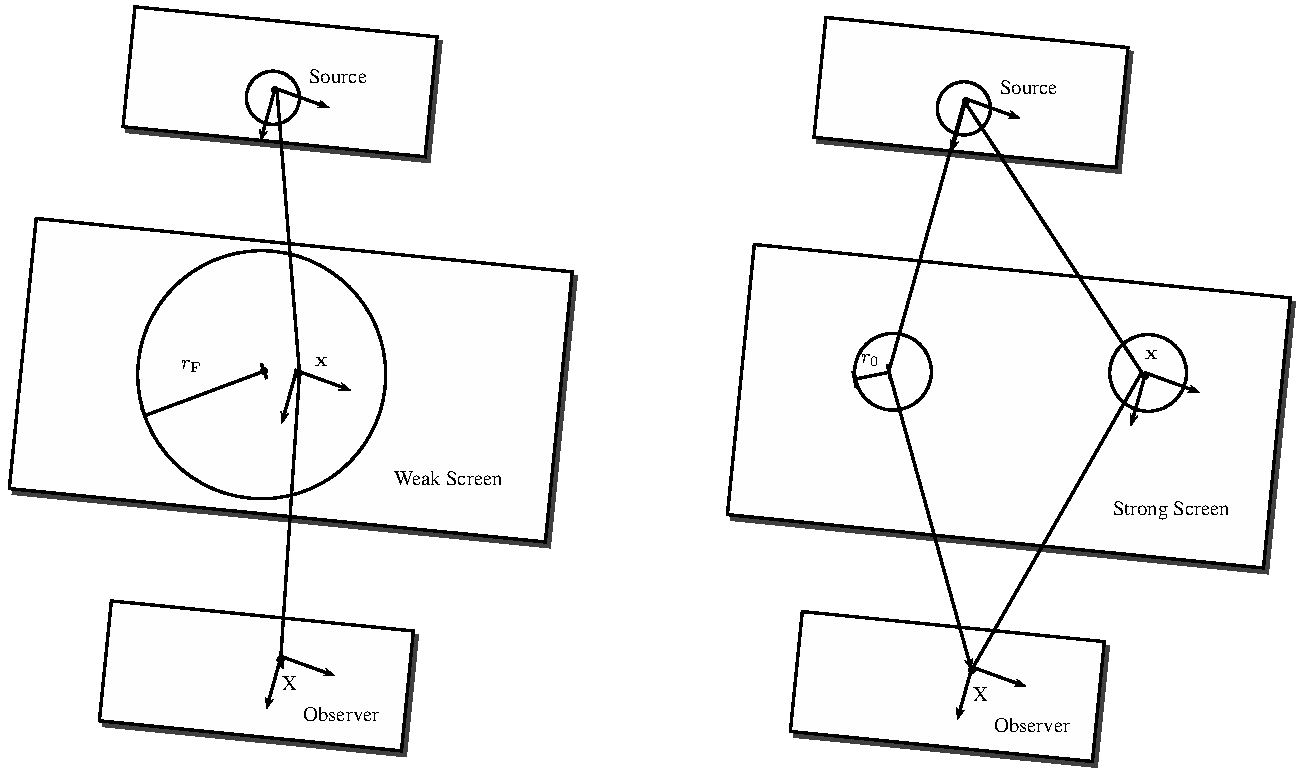
\includegraphics[width=1.\columnwidth]{Images/scatter.pdf}
\caption{Illustration depicting the basics of scattering in the weak (left) and strong (right) regimes. In the weak regime, the signal is coherently propagated over an area, $A_{\rm weak} \approx \pi r_{\rm F}^2$, whereas in the strong regime, coherent propagation is split over many areas, each of size $A_{strong} \approx \pi r_{\rm 0}^2$. \label{fig:scatter}
}
\end{center}
\end{figure*}

%frozen screen
To evolve the screen in time, we assume a frozen screen model i.e. that the velocity of the individual turbulent eddies is dominated by the bulk motion of scattering medium \citep[e.g.][]{Lay_1997}. This allows us to treat the screen as frozen but advected over the observer by a uniform motion. Hence, time variability can be easily incorporated by the relative motion between source, scattering screen, and observer.

\subsection{Interstellar medium scattering}\label{sec:ism_scat}
%PR 1 St 1 

%introduction and plan
Electron density inhomogeneities in the interstellar medium (ISM) plasma scatter the radio waves propagating through it, increasingly so towards the Galactic Centre. Radio interferometric observations of Sgr~A$^\star$ have characterised the basic properties of the intervening plasma material, however extensive developments in scattering theory and simulations have proved essential to the interpretation of more subtle scattering phenomena. This section begins with previous VLBI results which studied the Gaussian blurring effect of the scattering of Sgr~A*. We then expand on the scattering theory introduced in Sec.~\ref{sec:basic_scat} to review the latest theoretical developments which explore the presence of scattering-induced substructure. Finally, we review recent observational results which account for scattering substructure in their data interpretation. 


%blurring
The dominant observational effect of this scattering scenario for $\lambda \gtrsim 1$~cm is to convolve the intrinsic source structure with an elliptical Gaussian. The size of the Guassian exhibits a $\lambda^2$ scaling dependence over several orders of magnitude \citep[Fig.~\ref{fig:scattering_law}][]{Backer_1978, Shen_2005, Bower_2006, Lu_2011},which is consistent with the wavelength dependence of the refractive index of a plasma. In order to determine the parameters of the scattering kernel, i.e. major axis, minor axis and position angle,  one has to observe at wavelengths where the angular size of scattering ellipse is much larger than the expected source size. A Very Long Baseline Array (VLBA) + Green Bank Telescope (GBT) campaign  estimated the size at $1.31 \times 0.64$~mas cm$^{-2}$, oriented $78^\circ$ east of north \citep{Bower_2006}. 


%debluring,uncertainties of the extrapolation
An accurate extrapolation of the scattering kernel to 1.3~mm is important for the EHT scattering-mitigation strategy \cite{Fish_2014} which aims to deblur the scattered image through a deconvolution procedure. However as this extrapolation is over at least an order of magnitude, any small systematic error in the original measurement can significantly effect the 1.3~mm extrapolated parameters. A recent review of VLBI observations of Sgr~A$^\star$ \cite{Psaltis_2015} has noted that there are significant inconsistencies between different measurements. The authors used a Bayesian methodology to re-analyse the datasets resulting in increased uncertainties as shown in table~\ref{tab:ism_gauss}. The minor axis has a much larger uncertainty than the major axis due to the limited north-south coverage of the VLBA array. 
%fig showing power laws of scattering and intrinsic source
\begin{figure*}
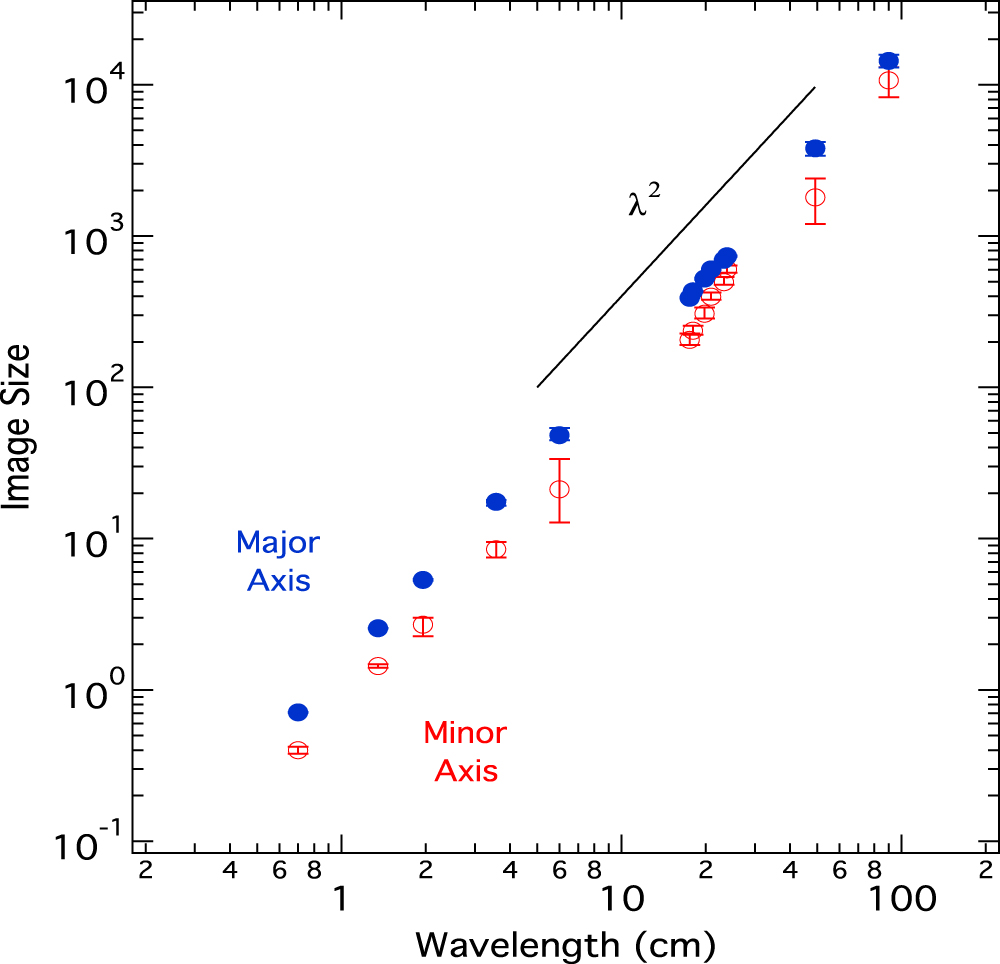
\includegraphics[width=0.6\columnwidth]{Images/scattering_law}
\caption{The $\lambda^2$ dependence of scattering kernel size is shown by the solid line. This has been derived from measurements made at $\lambda > 17$~cm \protect\cite{Bower_2006}. The dotted line shows the derived intrinsic source size which scales as $\lambda^{1.44}$. This was derived from measurements in the wavelength range, 2~cm~$< \lambda < 1.3$~mm \citep{Doeleman_2008}. The red circles show major-axis observed sizes of Sgr~A$^\star$  and the green points show the derived intrinsic major-axis size. This plot was reproduced from \protect\citet{Doeleman_2008}.\label{fig:scattering_law}
}
\end{figure*}
%table showing latest scattering kernel parameters
\begin{table}[]
\centering
\caption{A re-analysis of VLBI observations of Sgr~A$^\star$ by \citet{Psaltis_2015} has yielded revised estimates of the parameters associated with the Gaussian scattering kernel. Note that the position angle is measured East of North. \label{tab:ism_gauss}}
\begin{tabular}{l|ll}
\hline
major axis FWHM (mas/cm$^-2$)& 1.32 & 0.04 \\
minor axis FWHM (mas/cm$^-2$)& 0.82 & 0.21 \\
position angle ($^\circ$)& 77.8 & 9.7\\  
\hline
\end{tabular}
\end{table}


%theory - refractive scale and size of blurred image
The blurring effect can explained by the simple scattering model introduced in  Sec.~\ref{sec:basic_scat}. Recall, that in the strong scattering regime EM waves propagate from coherent patches with linear size $\sim r_0$, assuming a point source. Each patch will emit light coherently into a single-slit diffraction cone of angular size $\theta_{\rm scatt} \sim \lambda /r_0$. An observer will hence be illuminated by many patches spanning $\theta_{\rm scatt}$, yielding a blurred and broadened image, with projected size on the screen equal to the \emph{refractive scale},
\begin{equation}
r_{\rm ref} = \theta_{\rm scatt} D_{\rm os} = r_{\rm F}^2/r_0.
\end{equation}
$r_{\rm ref}$ is the third fundamental length scale in the strong scattering regime and is associated with the refractive timescale,
\begin{equation}
t_{\rm ref} = r_{\rm ref}/v,
\end{equation}
where $v$ is bulk, transverse velocity of the screen.
%calculating r_0 given \theta_scatt 
We can calculate $r_0$ given the FWHM of $\theta_{\rm scatt}$ through the more precise relation
\begin{equation}\label{eq:theta_scatt}
 \theta_{\rm scatt} = \frac{2\sqrt{2\ln{2}}}{2\pi} \lambda / r_0 (M+1)
\end{equation} 
where $M = D_{\rm os}/R$ is the magnification factor and $R$ is the source-screen distance. The magnification factor is a correction to the model introduced in Sec.~\ref{sec:basic_scat} when $R \approx \infty$ no longer holds and should be used when calculating distances in the observer plane \citep*{Goodman_1989}.
%Locating the scattering screen Bower 2014
The location of the scattering medium was originally thought to be in the Galactic Centre itself (within $\le 1$~kpc). However, observations of a newly discovered pulsar, SGR~J1745-29, indicate that the scattering screen is located at a distance $D_{\rm os} = 5.8 \pm 0.3$~kpc, within the Scutum spiral arm \citep{Bower_2014}. Using Eq.~\ref{eq:theta_scatt} and the parameters given in table \ref{tab:ism_gauss}, we find that the major axis of the coherence length at 1.3~mm, $r_0 \approx 3100$~km (i.e. 0.25 Earth diameters).


%shift to looking at refractive effects,theory, 3 regimes of scattering
Recent EHT and space-VLBI observations have shifted focus away from the well-studied Gaussian convolution effect of ISM scattering and onto the presence of stochastic scattering-induced substructure \citep[e.g.][]{Johnson_2016}. To understand this phenomenon, we must first develop the theory to be sensitivity to the averaging effects of the observation. 

Strong scattering can be further subdivided into \emph{snapshot}, \emph{average} and \emph{ensemble-average} regimes \citep*{Narayan_1989,Goodman_1989}. To understand the different regimes, remember that for each point on the source, the observer sees emission from coherent patches of area $A_{\rm strong} \sim \pi r_0^2$ over a total area $A_{\rm ref} \sim \pi r_{\rm ref}^2$. The diffraction cones from each of the patches will interfere, resulting in a \emph{diffractive scintillation} pattern, analagous to the classic multi-slit experiment. 

%snapshot regime
In the \emph{snapshot regime}, a compact source is observed with a narrow bandwidth and over a short time integration. This yields a single realisation of the diffractive scintillation pattern. By averaging over many snapshots, diffractive scintillation is quenched. This occurs if the source size $\theta_{\rm src}$ is much larger than the diffractive scale $\theta_{\rm src} \gg r_0/D_{\rm os}$; if the fractional bandwidth $\delta \nu/\nu$ is much larger than the decorrelation bandwidth $\delta \nu/\nu \gg \delta \nu_{\rm dc}/\nu \approx (r_0/r_{\rm F})^2$ \citep{Narayan_1992}; or if the integration time $t_{\rm int}$ is much larger the diffractive timescale $t_{\rm int} \gg t_{\rm 0} = r_0/v$, where $v$ is the relative velocity between screen, source and observer. This regime is hence only accessible through observations of compact objects like pulsars. On a side note, observations in this regime can be used to probe the source with angular resolution $\sim \lambda /r_{\rm ref}$ \citep[e.g.][]{Gwinn_2012}. This is because the scattering screen is essentially a lens of diameter $\approx r_{\rm ref}$.

%average regime 
In the \emph{average regime}, diffractive scintillation has been averaged over, however there still exists scintillation over scales comparable to the size of the scattered image of a point source $\sim r_{\rm ref}$, termed \emph{refractive scintillation}. Phase fluctuations on this scale act like a weak lens to focus or defocus the $\lambda/ r_0$ scale diffraction cones in the direction of the observer. For a point source this would lead to weak flux variations in the total flux \citep{Narayan_1992}. We will show later that refractive scintillation leads to the presence of substructure for a resolved scatter-broadened source. In contrast to diffractive scintillation, refractive scintillation is much more difficult to average over. Typically the refractive time scale $t_{\rm ref} = r_{\rm ref}/v$ is on the order of weeks to months for scattering towards the Galactic Centre i.e. longer than an observation campaign; the fractional decorrelation bandwidth is on the order of unity $\delta \nu_{\rm dc}/\nu \sim 1$ (c.f. EHT $\sim 1-10$\%; and the source has to be much larger than the image of a scattered point source $\theta_{\rm src} \gg \theta_{\rm scatt} \sim 10 \mu$-arcsec at $\lambda = 230$~GHz. 

%ensemble average
In the \emph{ensemble-average regime}, both diffractive and refractive scintillation have been averaged over. It is in this regime when  the scattering is equivalent to Gaussian convolution which is deterministic and not time variable. 


%approximation of the scattered image by Johnson 2015
A recent theoretical work \citep*{Johnson_2015a} has derived a useful approximation of the resolved scattered image $I_{\rm ss}$ in the average regime,
\begin{equation}\label{eq:scatterbrane}
I_{\rm ss}(\bm{x}) \approx I_{\rm src}\left(\bm{x} + r_{\rm F}^2 \nabla \phi(\bm{x})\right),
\end{equation}
where $\nabla$ is the directional derivative. Here we have used the same two-dimensional coordinate system, indexed by $\bm{x}$ to describe the source, screen and observer planes which are considered to be aligned along the vertical axis. The scattered image $I_{\rm ss}$ is approximated by a `reshuffling' of the source image $I_{\rm src}$. As $|\nabla\phi| \sim 1/r_0$, the magnitude of the translation of points on $I_{\rm src}$ $\sim r_{\rm ref} \sim 10\ \mu$-arcsec in the case of Sgr~A$^\star$ at 1.3~mm. 

%Coherence of the phase slope 
Even though $\phi(\bm{x})$ is only coherent to $\sim r_{\rm 0}$, $\nabla \phi(\bm{x})$ remains spatially coherent over much larger scales. The autocovariance of the phase derivative can be related to the structure function \citep*{Johnson_2015a}
\begin{equation} 
\langle [ \partial_x \phi(\bm{x_0})] [ \partial_x \phi(\bm{x_0}+\bm{x})] \rangle = \partial_x^2 D_\phi(\bm{x}).
\end{equation}


A generalised structure function \citep{Tatarskii_1971, Narayan_1989} is quadratic ($r^2$) at small scales ($r<< r_{\rm in}$), Kolmogorov in the range $r_{\rm in}<r<r_{\rm out}$ and constant for $r>r_{\rm out}$. Taking the simplifying case of $r_{\rm in} \gg r_0$ and $r_{\rm in}<r<r_{\rm out}$ $D_\phi$ becomes \citep{johnson_dissertation},
\begin{equation}
D_\phi = \frac{2}{\beta}\left( \frac{r_{\rm in}}{r_0}\right)^{2-\beta} \left( \frac{r}{r_0}\right)^\beta, 
\end{equation}
and, 
\begin{equation}
 \partial_r^2 D_\phi(\bm{r}) \propto r^{\beta-2}.
\end{equation}

Therefore in the Kolmogorov regime ($\beta = 5/3$), the coherence of image shift relative to the refractive scale $\propto (r/r_0)^{-1/3}$. Therefore, even though $\phi(\bm{x})$ is only coherent to $\sim r_{\rm 0}$, $\nabla \phi(\bm{x})$ remains spatially coherent over much larger scales, leading to the presence of refractive substructure \citep*{Johnson_2015a}.

%Observations of substructure
A recent observation of Sgr~A$^\star$ at 3.5~mm by the VLBA+LMT \citep[see Fig.~\ref{fig:substructure2}][]{Ortiz_2016} has measured non-zero closure phases on its longest baselines. However it was also shown in the data anaylsis that the measured values are consistent with expectation refractive scintillation assuming a circular Gaussian source of FWHM~$=130\ \mu$-arcsec, which is the fitted size of the major axis of the intrinsic source emission. Another observation at 1.3~cm shows flux amplitude variability due to scattering substructure $\Delta S \sim 10$~mJy \citep{Gwinn_2014}. Predictions for $\lambda = 1.3$~mm show $\sim 60$~mJy for long East-West baselines and $\sim 25$~mJy for long North-South baselines \citep*{Johnson_2015a}, assuming a Gaussian source of FWHM~$=40\ \mu$-arcsec.


\begin{table}[h!]
\begin{tabular}{c}
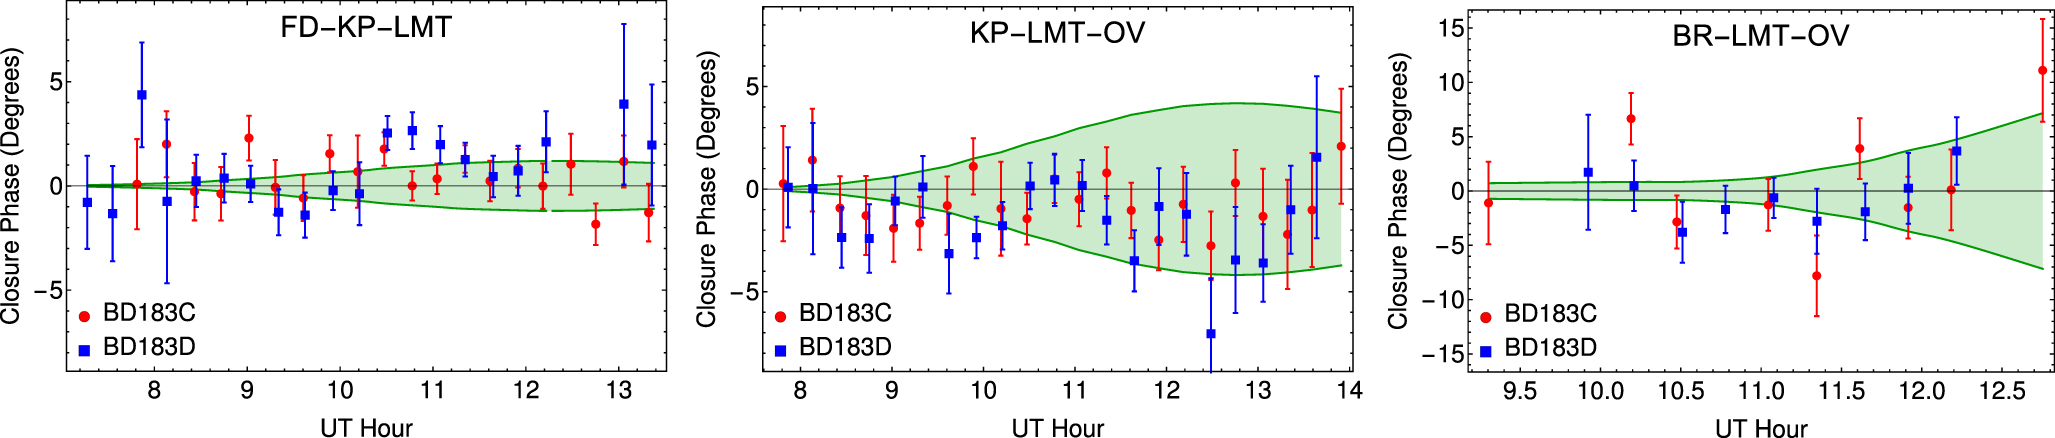
\includegraphics[width=\columnwidth]{Images/ism_cp}\\
\hline
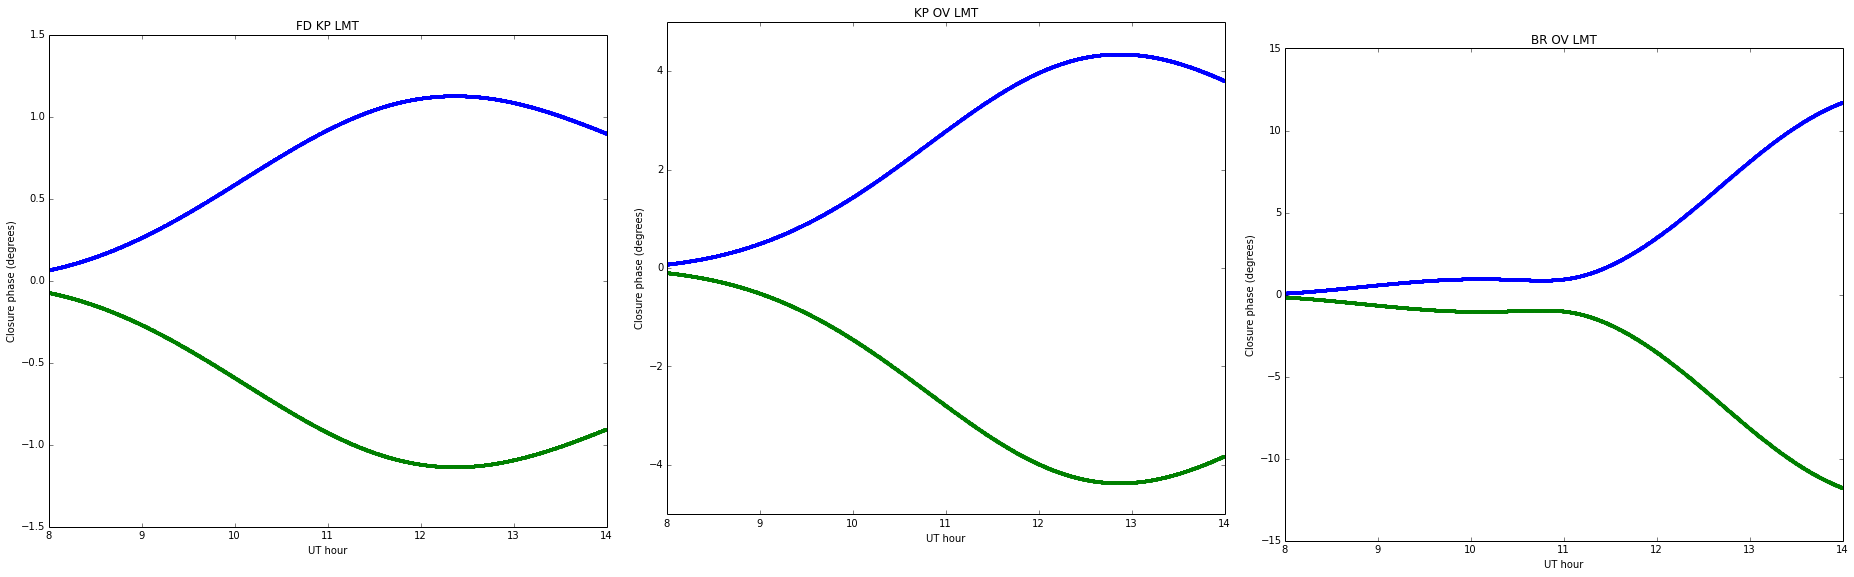
\includegraphics[width=\columnwidth]{Images/ortizrepeat}\\
\end{tabular}
\caption{{\bf Top panel :} Closure phases recorded in a VLBA + LMT observation of  Sgr~A$^\star$ at $\lambda = 3.5$~mm \protect\cite{Ortiz_2016}. The data points are shown as red circles and blue squares and are only distinguished by the calibrator used. The green envelopes show the $1\sigma$ closure phase prediction induced by scattering-induced substructure. The prediction was generated by simulating interferometric observations of 500 independent realisations of a scattered circular Gaussian with FWHM~$=130\ \mu$-arcsec. Reproduced from \protect\citet{Ortiz_2016}. {\bf Bottom panel :} Reproduction of the above result using the {\sc meqsilhouette} simulator using 50 independent realisations of the scattering screen. The success of the reproduction confirms the functionality of a large section of the simulator.\label{fig:substructure2}
}

\end{table}


%Distinguishing intrinsic source structure and variability
Distinguishing intrinsic source and ISM substructure and variability is an interesting challenge. Observations at mm-wavelengths have revealed deviations from the $\lambda^2$ scattering scaling law, see Fig.~\ref{fig:scattering_law}. This is interpreted as due to the presence of intrinsic source structure and has been fitted with a power-law with an exponent of $1.34 \pm 0.01$ \cite{Lu_2011}. This has enabled the constraint of various theoretical models \cite{Bower_2006}, excluding advection-dominated accretion flows (ADAF) \cite{Narayan_1998} and Bondi-Hoyle accretion \cite{Melia_1994}. However observations extending over month timescales are required to properly sample the larger scale inhomogeneities and even with multiple epoch observations, it can be difficult to distinguish source and scattering characteristics \citep*{Macquart_2006}. The developments in scattering theory presented above provide a robust mechanism for quantifying refractive effects. This could allow a decoupling without sampling a refractive ensemble but significant assumptions are always made on the source model. 


\subsection{Troposphere}\label{sec:trop}
%PR 1 St 1

%Introduction - Troposphere is a problem. Define troposphere. st 1
The coherence and intensity of millimetre wavelength electromagnetic waves are most severely deteriorated in the lowest atmospheric layer, the troposphere which extends up to an altitude of $7-10$~km above sea level and down to a temperature $T \sim 218$~K \citep{Thompson_2001}. The troposphere is composed of a number of different components including primary gases $\rm N_2$ and  $\rm O_2$, trace gases e.g. water vapour and ${\rm CO_2}$, as well as particulates of water droplets and dust. The rest of this section will explore the tropospheric corruption for the mm-VLBI case beginning with insights from the fundamentals of electromagnetic propagation, followed by a review of atmospheric corruptions in the sub-mm regime. We then firm up our theory with a discussion on atmospheric radiative transfer and atmospheric turbulence. 


\subsubsection{Propagation fundamentals}\label{sec:prop_fund}
%propagation fundamentals st 1
Consider a quasi-monochromatic wave passing through a linear medium,
\begin{equation}
E_\nu(x,t) = E_0 \exp^{i(kn_\nu x - 2\pi\nu t)},
\end{equation}		
where $k=2\pi \nu/c$ is the propagation constant in free space and $n= n_{\rm R} + j n_{\rm I}$ is the complex index of refraction. Note that we will occasionally omit the frequency dependence of $n$ and related quantities to simplify the notation. If $n_{\rm I}$ is nonzero, the electric flux $I$ will decay exponentially
\begin{equation}
I = EE^\ast = E_0^2 \exp(-\tau),
\end{equation}
where $\tau$ is called the opacity or optical depth and is related to the absorption coefficient, $d\tau = \kappa dx$ where $\kappa = 4\pi \nu n_I/c$. If $n_{\rm R} > 1 $ the phase velocity of the EM wave will decrease, $v_{\rm p} = c/n_{\rm R}$, which results in a time delay. The time delay due to the troposphere, $\tilde{t}$ and opacity $\tau$ can be calculated simultaneously,
\begin{equation}\label{timedelay}
\tilde{t} + i \tau /4\pi \nu =1/c \int_{path} d\bm{s}\  (n_\nu(\bm{s}) -1).
\end{equation}

%the relationship between delay-absorption-noise st 1
In the interferometric context opacity and time delay are often viewed independently. However, the electric field is real and causal which imposes restrictions on the complex refractive index. Specificially $n_{\rm R}$ and $n_{\rm I}$ contain the same information and can be interchanged via the Kramers-Kronig relations. 

Absorption is accompanied by emission and for a medium in local thermodynamic equilibrium, Kirchoff's law states that 
\begin{equation}\label{kirchoff}
\frac{\epsilon_\nu}{\kappa_\nu}=B_\nu(T),
\end{equation}
where $\epsilon_\nu = dI_\nu/dx$ is the emission coefficient and $B_\nu(T)$ is the Planck function. Hence the absorbing molecules are also emitters, and so non-zero opacity will lead to both absorption and emission, the latter of which will be seen by the receiver as an increased sky noise component, and hence an increase in total system temperature/noise. Therefore opacity, time delay and atmospheric noise are interrelated and should be simulated consistently. On a side note these relations allow for phase calibration using measurements of sky emission via Water Vapour Radiometry (WVR) \citep*[e.g.][]{Carilli_1999}.

\subsubsection{Atmospheric corruptions in the (sub-)mm regime}
%st 1
%Absorption in the GHz regime st 1
An analysis of the absorption spectrum in the GHz range (Fig.~\ref{fig:absorption}), shows that it is dominated by transitions of $\rm H_2O$ and $\rm O_2$ as well as a pseudo-continuum opacity which increases with frequency. The pseudo-continuum opacity is due to the cumulative effect of the far wings of a multitude of pressure-broadened water vapour lines above 1~THz \citep{Carilli_1999}. At 230~GHz the absorption is typically $5-10$\% at the best sites (e.g. Mauna Kea), during good weather . 

%Fig Absorption spectrum in the GHz st 1
\begin{figure*}
\begin{center}
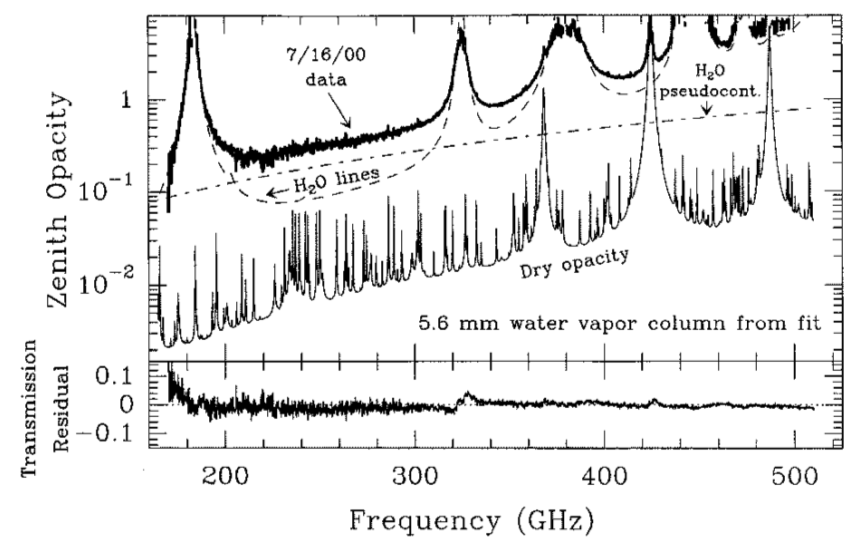
\includegraphics[width=\columnwidth]{Images/absorption}
\caption{Recorded zenith absorption spectrum in the $160-520$~GHz range, taken on Mauna Kea at an altitude of $\approx 4000$~m. The data has been fit to a sum of $\rm H_20$ lines, an $\rm H_20$ pseudo-continuum and dry absorption lines. The model has been generated using the \textsc{atm} code (see section~\ref{sec:atm_theory}), with the bottom panel showing the residuals. Here `dry' refers to all atmospheric constituents except $\rm H_20$. Reproduced from \citet{Pardo_2001} \label{fig:absorption}
}
\end{center}
\end{figure*}

%Phase variability in the GHz st 1
In contrast to the dry atmospheric components, water vapour mixes poorly and its time-variable spatial distribution induces rapid fluctuations in the time delays $\tilde{t}$ above each station. The phase error for a baseline (1,2) where antenna 1 is the reference will be
\begin{equation}\label{eq:phase_ref}
\delta \phi(t, \nu) = 2\pi/\nu(\tilde{t}_2(t, \nu) - \tilde{t}_1(t, \nu)).
\end{equation}
The water vapour column density is measured as the depth of the column when converted to the liquid phase and is referred to as the precipitable water vapour (PWV). PWV is directly proportional to the time delay and hence the phase delay, 
\begin{equation}
\delta\phi \approx \frac{12.6\pi}{\lambda} \times w, 
\end{equation}\label{eq:phi-pwv}

\noindent where $w$ is the depth of the PWV column \citep*{Carilli_1999} and an atmospheric temperature $T=270$~K has been assumed. This relationship between phase and water vapour content has been experimentally verified \citep{hogg_1981}. At 230~GHz, the change in PWV needed to offset the phase by 1~rad is $\Delta w\approx0.03$~mm (again, assuming $t=270$~K). 

This sensitive dependence of phase coherence on atmospheric stability is aggravated by three factors. Firstly, antenna elevation angles are typically fairly low for EHT observations which increases the atmospheric path length. Secondly, as stations are far apart ($\gg 100$~km~$\gg r_{\rm out}$) the atmospheric variations are uncorrelated between stations, this increases visibility decoherence as atmospheric variations appearing in both terms of equation~\ref{eq:phase_ref} fall away. Thirdly, observing with few stations gives less constraints on unknown complex gains and therefore a smaller fraction of retrievable instrinsic information \citep{Thompson_2001}.


\subsubsection{Radiative transfer}\label{sec:atm_theory}
%St 1

%Radiative transfer, how solving it will give observables in a self-consistent manner st 1
The problem of radiative transfer through a static atmosphere is well described and implemented by the Atmospheric Transmission at Microwaves (\textsc{atm}) software \citep{Pardo_2001}. \textsc{atm} has been incorporated into \textsc{MeqSilhouette} to provide a fast and sophisticated procedure to calculate average opacities, sky brightness temperatures and time delays. Here we provide a brief summary of the theory underpinning the package but refer the reader to \citet{Pardo_2001} for more detail. \textsc{atm} is commonly used in the Atacama Large Millimeter Array (ALMA) community \citep[e.g.][]{Curtis_2009,Nikolic_2013} and has been tested with atmospheric transmission spectra taken on Mauna Kea \citep{Serabyn_1998}.

%Radiative transfer st 1
We start from the unpolarised radiative transfer equation, which is unidirectional in the absence of scattering,
\begin{equation}\label{eq:rad_trans}
\frac{dI_\nu (s) }{ds} = \epsilon_\nu(s) -\kappa_\nu(s)  I_\nu (s),
\end{equation}
where $s$ is the coordinate along the signal path through the atmosphere. We assume local thermodynamic equilibrium (LTE) which should hold as the collisional timescale is much smaller than the time for spontaneous emission for all but the highest part of the atmosphere. Applying equation~\ref{kirchoff}, multiplying by $\exp(-\tau_\nu)$ and integrating from the top of the atmosphere ($s=0$) yields, 
\begin{equation}\label{eq:rad_trans2}
I_\nu(s) = I_\nu(0) e^{-\tau_\nu (0,s) }+ \int_0^s B_\nu(s')e^{-\tau_\nu (s',s) }\kappa_\nu(s')ds',
\end{equation}
where  $s'$ is a dummy variable in the same direction as $s$ and $\tau_\nu (0,s) = \int_0^{s} k_\nu(s')ds'$. $I_\nu(0)$ is normally taken as the radiance from the Cosmic Microwave Background (CMB).
To calculate the $I_\nu(s)$, $\tau(s)$ and complete the above integral, requires $\kappa_\nu$ as a function of altitude and frequency. The time delay $\tilde{t}$ can be calculated from $\tau$ using the Kramers-Kronig relations. 


%deriving the absorption coefficient st 1
A general equation to determine the absorption coefficient for a transition between a lower $l$ and upper $u$ states is given in \citet{Pardo_2001}. Here we merely point out that it should be proportional to the energy of the photon, $h\nu_{l \to u}$, the transition probability or Einstein coefficient, $ B_{l \to u}$, the line-shape, $f(\nu,\nu_{l \to u})$ and the number densities $N$ of electronic populations. Line profiles which describe pressure broadening (perturbations to the Hamiltonian due to the presence of nearby molecules) and Doppler broadening are used. The condition of detailed balance further requires that decays from the upper state are included yielding, $g_u B_{u \to l} =g_l B_{l \to u}$, where $g$ is the degeneracy of the electronic state. Putting this together we find,

\begin{equation}
\kappa(\nu) _{l \to u}  \propto  h\nu   B_{l \to u}  \left(\frac{N_l}{g_l}  -  \frac{N_u}{g_u} \right) f(\nu,\nu_{l \to u}),
\end{equation}

\noindent where the Einstein coefficients are calculated from the inner product of the initial and final states with the dipole transition operator,\begin{equation}\label{coefficient}
B_{l \to u} = \frac{2\pi}{3\hbar^2} |<u|\mu|l>|^2,
\end{equation}
where $|u>$, $|l>$,$|\mu>$ are the wavefunctions of upper and lower states and the dipole transition operator respectively. The number densities of the two states, $N_u$ and $N_l$ in local thermodynamic equilibrium (LTE) are simply related to the local number density and temperature via Boltzmann statistics, 
\begin{equation}
\frac{N_n}{N} = g_n \frac {\exp{-\frac{E_n}{kT}}}{Q},
\end{equation}
where the partition function, $Q = \sum_i g_i  \exp{-E_n/kT}$. 
%inner product st 1
Transition lines at radio wavelengths result from rotational state transitions. To calculate the inner product given in equation~\ref{coefficient}, operators which describe linearly symmetric rotors (e.g. ${\rm O_2}$, ${\rm CO}$) and asymetric rotors are used. The asymetric rotations are decomposed into three principal rotation axes with differing rotational constants governing each axis. Rotational constants were measured by the authors as well as drawn from a variety of literature. Partition functions and transition probability are calculated using approximations taken from the literature.
 

%lineshapes and pseudocontina st 1 
Far wing broadening of ${\rm H_2O}$ lines~$> 1.2$ THz extends to lower frequencies and is not completely represented by the line-shape used. This is believed to be due to self-self collisions of water molecules. Additionally there are terms from the dry atmosphere related to transient dipoles and Debye absorption which are not represented in the line-shape. To correct for these effects, two pseudocontina are used. These are modelled as a power law dependence on frequency, temperature and the molecular densities. 

%summarise radiative transfer and constrast to other approaches () basically Phenomenology  - gaussian
The treatment of radiative transfer in {\sc atm}, and hence {\sc meqsilhouette}, is aimed at being as physical as possible, which .   


\subsubsection{Turbulent phase fluctuations}\label{sec:turb_theory}
%St 1

%phase fluctuations as a calibration problem st 1
\begin{quotation}
``Visibility phase instability  $\delta \phi(t)$ due to tropospheric turbulence is a fundamental limitation to producing high dynamic range, high fidelity, science-quality maps with a mm-VLBI array \citep{Thompson_2001}. The coherence time-scale is typically too rapid ($\lesssim10$~s) for fast switching calibration, so other calibration procedures (e.g. water vapour radiometry, paired antennas, and/or self-calibration) must be performed. Self-calibration is the most commonly used but is limited by the integration time needed to obtain adequate SNR to fringe-fit (see section~\ref{sec:self_cal}). Phase decoherence often leads to the use of closure quantities to perform model fitting \citep{Doeleman_2001,Bower_2004, Shen_2005}, and causes a decrease in measured flux due to incoherent complex averaging.''\\
\citep{Blecher_2016}
\end{quotation}

%plan
In this section we will review and develop the weak scattering theory introduced earlier which will culminate in a formulation for the simulation of tropospheric phase turbulence seen by a mm-VLBI array. How this formulation is implemented and fits into the broader atmospheric simulation framework will be discussed in section~\ref{sec:trop_imp}. 


%Following from scattering intro, weak scattering model setup st 1
Following from section~\ref{sec:basic_scat}, we model the statistics of $\delta \phi(t)$ with a thin, frozen, Kolomogorov-turbulent phase screen moving with a bulk velocity, $v$. 
%Discussion on thickness of turbulent layer st3
However, the turbulent layer has a finite width $\Delta h$ and outer scale $r_{\rm out}$ and both Kolmorogov theory and measurement \citep[Fig.~\ref{fig:screentransition},][]{Coulman_1985, Treuhaft_1987, Carilli_1997} show that $\beta$ should move continously through approximately three regimes,
\begin{equation}
 \beta = \left\{
 \begin{array}{rl}
 5/3 & \text{if } r < \Delta h,\\
2/3 & \text{if } r > \Delta h,\\
0 & \text{if } r > r_{\rm out}.
 \end{array}
\right\}
\end{equation}

In Fig.~\ref{fig:screentransition} we can see estimations of $\Delta h \approx 1$~km and $r_{\rm out} \approx 6$~km. We will show later that even though we are working with a VLBI array, our implementation falls into the $r \ll \Delta h$ regime.


%Fig. Phase variability carilli_1997 st 1
\begin{figure*}
\begin{center}
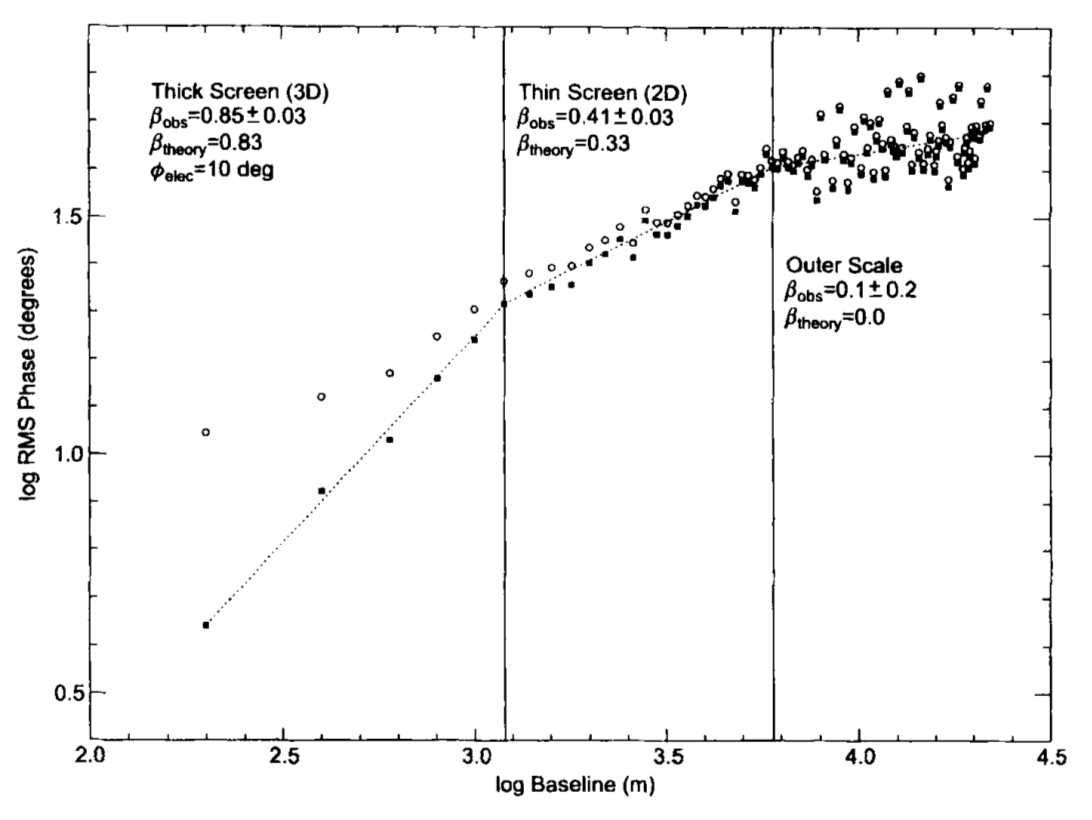
\includegraphics[width=\columnwidth]{Images/screentransition}
\caption{A log-log plot of RMS visibility phase versus baseline length for an observation of 1~Jy source 0748~+~240 with VLA at 22~GHz over a 90~min duration. The open circles show RMS phase as measured whereas the solid squares show the same values with a constant thermal noise contribution of $10^\circ$ subtracted in quadrature. Note that the measured and theoretical Kolmogorov turbulent exponent $\beta$ changes with distance on the phase screen as the viewing configuration transitions from a thick screen ($\beta_{\rm theory} = 5/3$) to a thin screen ($\beta_{\rm theory} = 2/3$) at $r \approx 1$~km and from a thin screen to completely uncorrelated regime ($\beta = 0$) beyond the outer scale at $r \approx 6$~km. Although these regimes appear distinct, there is continous variation between them. Reproduced from \citet*{Carilli_1997} \label{fig:screentransition}
}
\end{center}
\end{figure*}

 %weak scattering model setup st 1
\begin{quotation}
``We set the height $h$ of the screen at the water vapour scale height of 2~km above ground. At $1.3$~mm, the Fresnel scale is $r_F \approx 0.45$~m and experiments show annual variations of $r_0 \sim 50 - 500$~m above Mauna Kea \citep{Masson_1994} and $r_0 \sim 90 - 700$~m above Chajnantor \citep*{Radford_1998}, where both sites are considered to have excellent atmospheric conditions for (sub)millimetre astronomy. As $r_F < r_0$, this is an example of weak scattering. 


%simplifying the scattering model st 1
The required field-of-view (FoV) of a global mm-VLBI array is typically $FWHM < 1$~marcsec or $\sim10~\mu$-m at a height of 2~km, which is roughly 7-8 orders of magnitude smaller than the tropospheric coherence length. The tropospheric corruption can therefore be considered constant across the FoV and, from the perspective of the Measurement Equation, modeled as a diagonal Jones matrix per time and frequency interval. As VLBI baselines are much longer than the coherence length, $|\bm{b}| \ge 1000$~km~$\gg \rm r_0$, the phase screen at each site must be simulated independently. This assumption only holds for VLBI baselines and the framework needs to be extended to simulate the effects of turbulence on individual phased arrays stations (e.g. SMA) and short ($<10$~km) baselines (e.g. JCMT - SMA).'' 
\citep{Blecher_2016}
\end{quotation}
In principle, this could be approximated by assuming a time-variable phase efficiency for the phased array stations, however this is for future work.

\begin{quotation}
%structure function formulation st 1
``Our aim then is to produce a phase error time sequence $\left\{\delta \phi(t_i)\right\}$ for each station which is added to the visibility phase. We invoke the frozen screen assumption and write the structure function as a function of time, ${D (t) =  D(r)|_{r=vt}}$. The temporal structure function $D(t)$ provides an efficient route to sample the variability of the troposphere at the typical integration time of the dataset, $t_{\rm int} \sim 1$~sec. 

The temporal variance of the phase is a function of the temporal structure function, and accounting for time integration yields \citep*[see][B3]{Treuhaft_1987} 

\begin{equation}
\sigma^2_{\phi}(t_{\rm int}) = (1/t_{\rm int})^2 \int_{0}^{t_{\rm int}} (t_{\rm int}-t) D_{\phi}(t) dt.
\end{equation}

Assuming power-law turbulence and integrating yields, 

\begin{equation}\label{eq:turb_final}
\sigma^2_\phi (t_{\rm int})=\left[\frac{1}{\sin\theta(\beta^2 +3\beta +2)}\right]\left(\frac{t_{\rm int}}{t_0}\right)^{\beta},
\end{equation}


\noindent where $t_0 = r_0/v$ is the coherence time when observing at zenith and $1/\sin\theta$ is the approximate airmass which arises as $D_\phi \propto w$. As $r \ll \Delta h$, where $\Delta h$ is the thickness of the turbulent layer, an thin screen exponent of $\beta = 5/3$ is justified \citep*{Treuhaft_1987}. The phase error time-series takes the form of a Gaussian random walk per antenna. At mm-wavelengths, the spectrum of water vapour is non-dispersive up to a few percent \citep{Curtis_2009} and so we can assume a simple linear scaling across the bandwidth.


%A comparison to the phase screen approach st 1
Phase fluctuations $\delta\phi(t)$ can also be simulated by taking the inverse Fourier transform of the spatial phase power spectrum. However this approach is much more computationally expensive, e.g. for an observation length $t_{\rm obs}$ involving $N_{\rm ant}=8$ independent antennae with dish radii $r_{\rm dish}=15$~m, wind speed $v=10$~m\,s$^{-1}$ and pixel size equal to $r_{\rm F}$, the number of pixels $N_{\rm pix} \approx N_{\rm ant} t_{\rm obs} r_{\rm dish}^2/(v r_{\rm F}^3)  \sim 10^8$. Additionally, due to fractal nature of ideal Kolmogorov turbulence, the power spectrum becomes unbounded as the wavenumber approaches zero which makes it difficult to determine the sampling interval of the spatial power spectrum \citep{Lane_1992}.''\\
\citep{Blecher_2016}
\end{quotation}

\subsection{Instrumental}

%plan
All instruments suffer from both systematic and stochastic errors, the characterisation of which determines the measurement accuracy and precision respectively. In this section we explore thermal noise (stochastic) and antenna pointing errors (systematic). 
%completeness and classes of corruptions
While there are many additional potential sources of error (e.g. clock errors, bandpass, polarisation leakage, phasing errors, quantisation, correlator model, etc.), the primary aim here is to demonstrate the mm-VLBI framework that enables more sophisticated interferometric simulations. The Measurement Equation formalism enables any arbitrary linear error to be incorporated as a Jones Matrix, for example, a bandpass error would be a frequency-dependent diagonal Jones matrix.

\subsubsection{Thermal Noise}
%Pr 1 St 1


%Mild derivation of the thermal noise equation.
The level of thermal noise of the measurement defines the absolute limit on the sensitivity of the interferometer to detect a source and also to distinguish fine source characteristics. Closure quantities are especially prone to high levels of thermal noise as several visibilities are multiplied with one another. The thermal noise of an interferometer can be derived by correlating the thermal noise of two antennae \citep*{Wrobel_1999}. The  RMS thermal noise of an interferometer $\{i,j\}$, over a bandwidth $\Delta \nu$, for a single polarisation and over an integration time $t_{\rm int}$ is given by 

\begin{equation}
 \Delta S_{\rm ij} = \frac{1}{\eta_{\rm s}}\sqrt{\frac{SEFD_{\rm i}\ SEFD_{\rm j}}{2 \Delta \nu t_{\rm int}}},  
\end{equation}
where $\eta_{\rm s}$ is the system efficiency and $2 \Delta \nu t_{\rm int}$ is the number of independent samples. The $SEFD$ is a measure of the sensitivity of an antenna, accounting for the effiency, collecting area and thermal noise and is defined as the flux density of a source with the same power,
\begin{equation}
 SEFD = 2 k_{\rm B} T_{\rm sys} / (\eta_{\rm a} A),
\end{equation}
where $A$ is the antenna area, $\eta_{\rm a}$ is the antenna efficiency, $T_{\rm sys}$ is the system temperature and the factor $\frac{1}{2}$ accounts for only sampling 1 polarisation.


% Link to RIME -> additive matrix
As the RIME was formulated for a thermal noise-free measurement, we do not apply this corruption as a multiplicative matrix but rather an additive matrix,
\begin{equation}\label{eq:noise_matrix}
\bm{V}_{pq} = \bm G_p \bm{X}_{pq} \bm G_q^H + \bm N_{pq},
\end{equation}
where each component of $N_{pq}$ is sampled from a complex-valued Gaussian distribution of mean and variance, $|N_{pq}| \sim (0, \Delta S_{\rm ij}^2)$.


\subsubsection{Antenna Pointing}\label{sec:point_theory}
%Pr 1 St 1


%A bit more info on E-Jones terms - put it in the RIME

%Intro
\begin{quotation}
``All antennas suffer pointing errors to some degree due to a variety of factors including dish flexure due to gravity, wind and thermal loading, as well as drive mechanics. This corresponds to an offset primary beam, which should only translate to minor amplitude errors if the pointing error $\theta_{\rm PE}$ is significantly smaller than the primary beam (i.e. $\theta_{\rm PE} \ll \theta_{\rm PB}$). In the Measurement Equation formalism, this offset can be represented by a modified (shifted) primary beam pattern in the {\bf \it E}-Jones term \citep[see][]{Smirnov_2011a}
\begin{equation}
{\bf E}_p(l,m) = {\bf E}(l_0 + \delta l_p, m_0 + \delta m_p),
\end{equation}
where $\delta l_p, \delta m_p$ correspond to the directional cosine offsets.''\\
\citep{Blecher_2016}
\end{quotation}

%Motivation, why this could be a problem for mm observations
This could be a problem for millimetre observations as the primary beam is narrow. For example, at an observing frequency of 230~GHz, the primary beam of a 30~m dish is $\theta_{\rm PB} \sim 10$~arcsec. The typical pointing budget for millimetre stations are $\theta_{\rm PE} \sim 1$~arcsec.

% Different categories of pointing error i.e. tracking vs slew

We identify two main classes of pointing error. Firstly, an antenna tracking a source could suffer a slow, continuous time-variable pointing error associated with the tracking error $\sigma_{\rm track}$. Physically, this could be attributed to changes in wind, thermal and gravitational loading which all change with telescope pointing direction and over the course of a typical few hour observation. Using the {\sc meqtrees} software package, such behaviour has been demonstrated to occur with the Westerbork Synthesis Radio Telescope \citep[WSRT,]{Smirnov_Calim_2011,Smirnov_2011c}).


Secondly, whilst a stationary phase centre is tracked, the pointing error should evolve slowly and smoothly, however, in mm-VLBI observations the phase centre is often shifted to another source/calibrator. This would cause the pointing error to change abruptly, with an absolute pointing error $\sim \sigma_{\rm abs}$. Source/calibrator change is scheduled every 5-10 minutes in a typical millimetre observation. The point is that even though EHT will be able to determine the pointing offset when observing a calibrator with relatively well-known structure, when the antennas slew back to a source (e.g. Sgr~A$^\star$) with less certain or variable source structure, the pointing error could change significantly. This is exacerbated by the scarcity of mm-wavelength calibrators, which are often widely separated from the source.
